\section{Government}
	\subsection{Registration}
	The government cannot register a new account like other citizens and 
	businesses and only one account is allowed. This account is provided 
	by the developer of \textit{Soldino}.
	\subsection{Login}
	If you already have a personal account press the "login" button on the 
	top right of the homepage, you will automatically log in your account 
	(there is no need for a username or password, all is done via MetaMask). 
	\\To be able to log in you have to be logged in your MetaMask account.
	\subsection{Logout}
	To log out of \textit{Soldino} you just have to log out of 
	your MetaMask. To do this you have to press MetaMask's icon on the top 
	right of the browser, press your account's icon and then press "Log out"
	on the top right.
	\begin{figure}[H]
		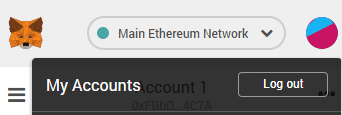
\includegraphics[width=7cm]{res/images/logout_metamask.png}
		\centering
		\caption{Logging out}
	\end{figure}
	\subsection{Cubit}
		\subsubsection{Minting}
		The Government can mint Cubits, a special token for \textit{Soldino} 
		that has the value of 1 Euro. This can be done by visiting 
		
		\subsubsection{Distributing}
		Government can distribute Cubits previously minted amongst the users of 
		the platform. This can be done by visiting 
		
%	\subsection{Managing users}
%	The Government can activate disabled accounts or deactivate active accounts.
%	This can be done by visiting the page containing all users.
%		\subsubsection{Activating users}
%		After you have found the account you want to enable press the button 
%		"Enable". After being enabled an account will again be able make purchases
%		on \textit{Soldino}
%		
%		\subsubsection{Deactivating users}
%		After you have found the account you want to disable press the 
%		"Disable" button. After pressing it a window will open where you can 
%		write a	message explaining why the account was disabled that will be 
%		shown when that user will try an log in. Disabling an account 
%		means that it will not be able to make purchases on \textit{Soldino} 
%		until it is enabled.
		
	\subsection{Reimbursing businesses}
	The government can reimburse business of their VAT credit. This can be done 
	by visiting